\section{Durchführung}
\label{sec:Durchführung}
Als erstes wird die Güte Q des Selektivverstärkers bestimmt. Dafür wird eine Sinusspannung durch des Selektivverstärker hindurch gemessen. 
Die Frequenz dieser Spannung wird Schritt für Schritt von 20kHz bis 40kHz erhöht, während der Selektivverstärker auf $v_0$ = 3,5kHz und Q = 100 
eingestellt bleibt.
Anschließend wird die verwendete Sinussspannung durch ein Voltmeter bestimmt.
Danach wird eine Schaltung wie in Abbildung \ref{fig:3}, nur ohne den mittleren Verstärker aufgebaut.
Die Brückenspannung wird abgeglichen, der variierte Widerstand abgelesen, so wie die eingehende Spannung notiert.
Dann wird eine Probe in der Spule platziert, die nun eingehende Spannung notiert und die Brückenspannung wieder abgeglichen. 
Auch der nun gewählte Widerstand wird notiert ebenso wie die nun eingehende Spannung.
Diese Prozedur wird für zwei Proben je drei mal durchgeführt.

\begin{figure}
    \centering
    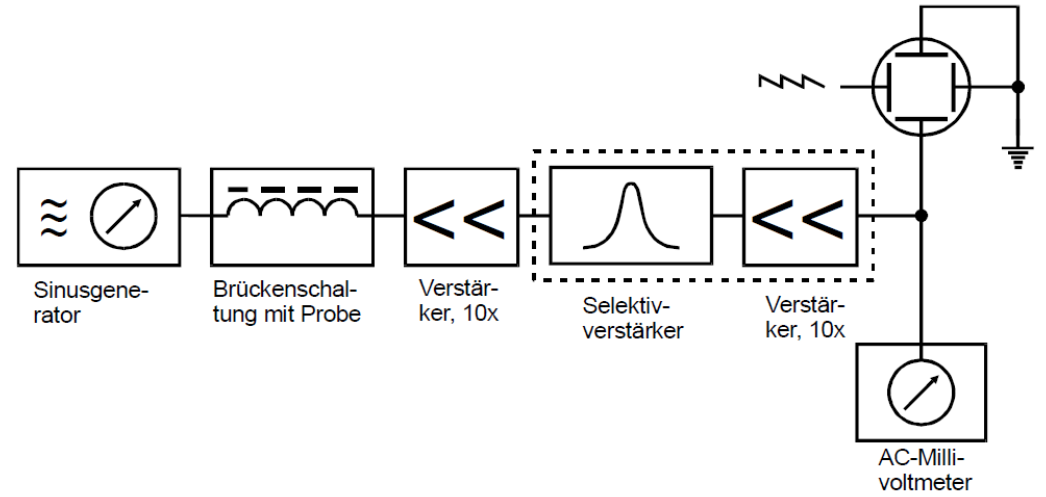
\includegraphics[width = 0.60\textwidth]{V606Bild3.png}
    \caption{Schematische Messschaltung.}
    \label{fig:3}
\end{figure}

